\documentclass{standalone}
\usepackage{tikz}
\usetikzlibrary{patterns, positioning}


\begin{document}
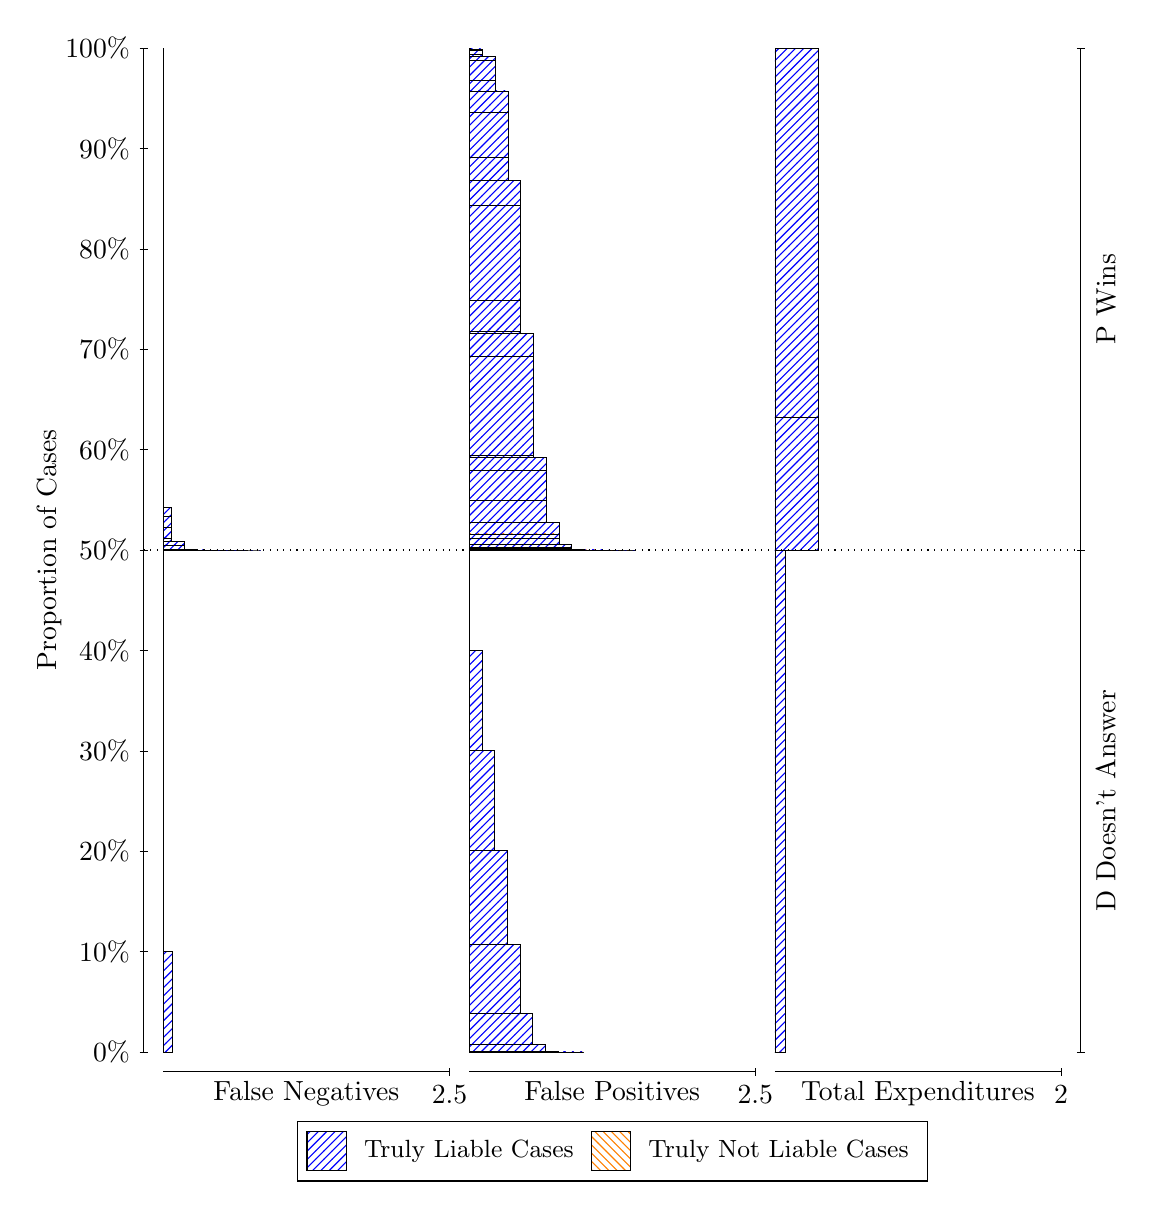
\begin{tikzpicture}
\draw[black, very thin] (1.5,1.75) -- (1.5,14.5);
\node[rotate=90, text=black, anchor=center] at (0.3, 8.125) {Proportion of Cases};
\draw[black, very thin] (1.45,1.75) -- (1.55,1.75);
\node[text=black, anchor=east] at (1.45, 1.75) {0\%};
\draw[black, very thin] (1.45,3.025) -- (1.55,3.025);
\node[text=black, anchor=east] at (1.45, 3.025) {10\%};
\draw[black, very thin] (1.45,4.3) -- (1.55,4.3);
\node[text=black, anchor=east] at (1.45, 4.3) {20\%};
\draw[black, very thin] (1.45,5.575) -- (1.55,5.575);
\node[text=black, anchor=east] at (1.45, 5.575) {30\%};
\draw[black, very thin] (1.45,6.85) -- (1.55,6.85);
\node[text=black, anchor=east] at (1.45, 6.85) {40\%};
\draw[black, very thin] (1.45,8.125) -- (1.55,8.125);
\node[text=black, anchor=east] at (1.45, 8.125) {50\%};
\draw[black, very thin] (1.45,9.4) -- (1.55,9.4);
\node[text=black, anchor=east] at (1.45, 9.4) {60\%};
\draw[black, very thin] (1.45,10.675) -- (1.55,10.675);
\node[text=black, anchor=east] at (1.45, 10.675) {70\%};
\draw[black, very thin] (1.45,11.95) -- (1.55,11.95);
\node[text=black, anchor=east] at (1.45, 11.95) {80\%};
\draw[black, very thin] (1.45,13.225) -- (1.55,13.225);
\node[text=black, anchor=east] at (1.45, 13.225) {90\%};
\draw[black, very thin] (1.45,14.5) -- (1.55,14.5);
\node[text=black, anchor=east] at (1.45, 14.5) {100\%};

\draw[black, very thin] (13.4,1.75) -- (13.4,14.5);
\draw[black, very thin] (13.35,1.75) -- (13.45,1.75);
\node[anchor=west] at (13.35, 1.75) {};
\draw[black, very thin] (13.35,8.125) -- (13.45,8.125);
\node[anchor=west] at (13.35, 8.125) {};
\draw[black, very thin] (13.35,14.5) -- (13.45,14.5);
\node[anchor=west] at (13.35, 14.5) {};

\draw[black, very thin, pattern color=blue, pattern=north east lines] (1.75,1.75) rectangle (1.859,3.025);
\draw[black, very thin, pattern color=orange, pattern=north west lines] (1.75,3.025) rectangle (1.75,3.025);
\draw[black, very thin, pattern color=blue, pattern=north east lines] (1.75,3.025) rectangle (1.75,8.125);
\draw[black, very thin, pattern color=blue, pattern=north east lines] (1.75,8.125) rectangle (2.9853,8.125);
\draw[black, very thin, pattern color=blue, pattern=north east lines] (1.75,8.125) rectangle (2.8239,8.125);
\draw[black, very thin, pattern color=blue, pattern=north east lines] (1.75,8.125) rectangle (2.8239,8.125);
\draw[black, very thin, pattern color=blue, pattern=north east lines] (1.75,8.125) rectangle (2.6624,8.125);
\draw[black, very thin, pattern color=blue, pattern=north east lines] (1.75,8.125) rectangle (2.5009,8.125);
\draw[black, very thin, pattern color=blue, pattern=north east lines] (1.75,8.125) rectangle (2.5009,8.125);
\draw[black, very thin, pattern color=blue, pattern=north east lines] (1.75,8.125) rectangle (2.3394,8.1256);
\draw[black, very thin, pattern color=blue, pattern=north east lines] (1.75,8.1256) rectangle (2.1779,8.1291);
\draw[black, very thin, pattern color=blue, pattern=north east lines] (1.75,8.1291) rectangle (2.1779,8.1373);
\draw[black, very thin, pattern color=blue, pattern=north east lines] (1.75,8.1373) rectangle (2.0164,8.1893);
\draw[black, very thin, pattern color=blue, pattern=north east lines] (1.75,8.1893) rectangle (2.0164,8.235);
\draw[black, very thin, pattern color=blue, pattern=north east lines] (1.75,8.235) rectangle (2.0164,8.235);
\draw[black, very thin, pattern color=blue, pattern=north east lines] (1.75,8.235) rectangle (1.855,8.2787);
\draw[black, very thin, pattern color=blue, pattern=north east lines] (1.75,8.2787) rectangle (1.855,8.4119);
\draw[black, very thin, pattern color=blue, pattern=north east lines] (1.75,8.4119) rectangle (1.855,8.5594);
\draw[black, very thin, pattern color=blue, pattern=north east lines] (1.75,8.5594) rectangle (1.855,8.6678);
\draw[black, very thin, pattern color=orange, pattern=north west lines] (1.75,8.6678) rectangle (1.75,8.6678);
\draw[black, very thin, pattern color=blue, pattern=north east lines] (1.75,8.6678) rectangle (1.75,14.5);
\draw[black, very thin, pattern color=orange, pattern=north west lines] (5.6333,1.75) rectangle (7.0867,1.75);
\draw[black, very thin, pattern color=blue, pattern=north east lines] (5.6333,1.75) rectangle (7.0867,1.75);
\draw[black, very thin, pattern color=blue, pattern=north east lines] (5.6333,1.75) rectangle (6.9252,1.7503);
\draw[black, very thin, pattern color=blue, pattern=north east lines] (5.6333,1.7503) rectangle (6.7637,1.7583);
\draw[black, very thin, pattern color=blue, pattern=north east lines] (5.6333,1.7583) rectangle (6.6022,1.8435);
\draw[black, very thin, pattern color=blue, pattern=north east lines] (5.6333,1.8435) rectangle (6.4407,2.2369);
\draw[black, very thin, pattern color=blue, pattern=north east lines] (5.6333,2.2369) rectangle (6.2793,3.1185);
\draw[black, very thin, pattern color=blue, pattern=north east lines] (5.6333,3.1185) rectangle (6.1178,4.3083);
\draw[black, very thin, pattern color=blue, pattern=north east lines] (5.6333,4.3083) rectangle (5.9563,5.5753);
\draw[black, very thin, pattern color=blue, pattern=north east lines] (5.6333,5.5753) rectangle (5.7948,6.85);
\draw[black, very thin, pattern color=blue, pattern=north east lines] (5.6333,6.85) rectangle (5.6333,8.125);
\draw[black, very thin, pattern color=orange, pattern=north west lines] (5.6333,8.125) rectangle (7.7407,8.125);
\draw[black, very thin, pattern color=blue, pattern=north east lines] (5.6333,8.125) rectangle (7.7407,8.125);
\draw[black, very thin, pattern color=orange, pattern=north west lines] (5.6333,8.125) rectangle (7.5792,8.125);
\draw[black, very thin, pattern color=blue, pattern=north east lines] (5.6333,8.125) rectangle (7.5792,8.125);
\draw[black, very thin, pattern color=orange, pattern=north west lines] (5.6333,8.125) rectangle (7.4177,8.125);
\draw[black, very thin, pattern color=blue, pattern=north east lines] (5.6333,8.125) rectangle (7.4177,8.1251);
\draw[black, very thin, pattern color=blue, pattern=north east lines] (5.6333,8.1251) rectangle (7.4177,8.1251);
\draw[black, very thin, pattern color=orange, pattern=north west lines] (5.6333,8.1251) rectangle (7.2562,8.1251);
\draw[black, very thin, pattern color=blue, pattern=north east lines] (5.6333,8.1251) rectangle (7.2562,8.1258);
\draw[black, very thin, pattern color=orange, pattern=north west lines] (5.6333,8.1258) rectangle (7.0947,8.1258);
\draw[black, very thin, pattern color=blue, pattern=north east lines] (5.6333,8.1258) rectangle (7.0947,8.1343);
\draw[black, very thin, pattern color=blue, pattern=north east lines] (5.6333,8.1343) rectangle (6.9333,8.1445);
\draw[black, very thin, pattern color=blue, pattern=north east lines] (5.6333,8.1445) rectangle (6.9333,8.1557);
\draw[black, very thin, pattern color=orange, pattern=north west lines] (5.6333,8.1557) rectangle (6.9333,8.1557);
\draw[black, very thin, pattern color=blue, pattern=north east lines] (5.6333,8.1557) rectangle (6.9333,8.1965);
\draw[black, very thin, pattern color=blue, pattern=north east lines] (5.6333,8.1965) rectangle (6.7718,8.2757);
\draw[black, very thin, pattern color=blue, pattern=north east lines] (5.6333,8.2757) rectangle (6.7718,8.3294);
\draw[black, very thin, pattern color=orange, pattern=north west lines] (5.6333,8.3294) rectangle (6.7718,8.3294);
\draw[black, very thin, pattern color=blue, pattern=north east lines] (5.6333,8.3294) rectangle (6.7718,8.4787);
\draw[black, very thin, pattern color=blue, pattern=north east lines] (5.6333,8.4787) rectangle (6.6103,8.7535);
\draw[black, very thin, pattern color=orange, pattern=north west lines] (5.6333,8.7535) rectangle (6.6103,8.7535);
\draw[black, very thin, pattern color=blue, pattern=north east lines] (5.6333,8.7535) rectangle (6.6103,9.1357);
\draw[black, very thin, pattern color=blue, pattern=north east lines] (5.6333,9.1357) rectangle (6.6103,9.3036);
\draw[black, very thin, pattern color=blue, pattern=north east lines] (5.6333,9.3036) rectangle (6.4488,9.3218);
\draw[black, very thin, pattern color=orange, pattern=north west lines] (5.6333,9.3218) rectangle (6.4488,9.3218);
\draw[black, very thin, pattern color=blue, pattern=north east lines] (5.6333,9.3218) rectangle (6.4488,10.59);
\draw[black, very thin, pattern color=blue, pattern=north east lines] (5.6333,10.59) rectangle (6.4488,10.872);
\draw[black, very thin, pattern color=blue, pattern=north east lines] (5.6333,10.872) rectangle (6.2873,10.897);
\draw[black, very thin, pattern color=blue, pattern=north east lines] (5.6333,10.897) rectangle (6.2873,11.292);
\draw[black, very thin, pattern color=orange, pattern=north west lines] (5.6333,11.292) rectangle (6.2873,11.292);
\draw[black, very thin, pattern color=blue, pattern=north east lines] (5.6333,11.292) rectangle (6.2873,12.501);
\draw[black, very thin, pattern color=blue, pattern=north east lines] (5.6333,12.501) rectangle (6.2873,12.815);
\draw[black, very thin, pattern color=blue, pattern=north east lines] (5.6333,12.815) rectangle (6.1259,12.815);
\draw[black, very thin, pattern color=blue, pattern=north east lines] (5.6333,12.815) rectangle (6.1259,13.115);
\draw[black, very thin, pattern color=blue, pattern=north east lines] (5.6333,13.115) rectangle (6.1259,13.688);
\draw[black, very thin, pattern color=blue, pattern=north east lines] (5.6333,13.688) rectangle (6.1259,13.957);
\draw[black, very thin, pattern color=blue, pattern=north east lines] (5.6333,13.957) rectangle (5.9644,13.957);
\draw[black, very thin, pattern color=blue, pattern=north east lines] (5.6333,13.957) rectangle (5.9644,14.091);
\draw[black, very thin, pattern color=blue, pattern=north east lines] (5.6333,14.091) rectangle (5.9644,14.346);
\draw[black, very thin, pattern color=blue, pattern=north east lines] (5.6333,14.346) rectangle (5.9644,14.39);
\draw[black, very thin, pattern color=blue, pattern=north east lines] (5.6333,14.39) rectangle (5.8029,14.424);
\draw[black, very thin, pattern color=blue, pattern=north east lines] (5.6333,14.424) rectangle (5.8029,14.469);
\draw[black, very thin, pattern color=blue, pattern=north east lines] (5.6333,14.469) rectangle (5.8029,14.488);
\draw[black, very thin, pattern color=blue, pattern=north east lines] (5.6333,14.488) rectangle (5.6414,14.499);
\draw[black, very thin, pattern color=blue, pattern=north east lines] (5.6333,14.499) rectangle (5.6414,14.499);
\draw[black, very thin, pattern color=blue, pattern=north east lines] (5.6333,14.499) rectangle (5.6333,14.5);
\draw[black, very thin, pattern color=orange, pattern=north west lines] (9.5167,1.75) rectangle (9.6529,1.75);
\draw[black, very thin, pattern color=blue, pattern=north east lines] (9.5167,1.75) rectangle (9.6529,8.125);
\draw[black, very thin, pattern color=orange, pattern=north west lines] (9.5167,8.125) rectangle (10.062,8.125);
\draw[black, very thin, pattern color=blue, pattern=north east lines] (9.5167,8.125) rectangle (10.062,9.8156);
\draw[black, very thin, pattern color=orange, pattern=north west lines] (9.5167,9.8156) rectangle (10.062,9.8156);
\draw[black, very thin, pattern color=blue, pattern=north east lines] (9.5167,9.8156) rectangle (10.062,14.5);
\draw[black, dotted] (1.5,8.125) -- (13.4,8.125);
\draw[black, very thin] (1.75,1.5) -- (5.3833,1.5);
\node[text=black, anchor=north] at (3.5667, 1.5) {False Negatives};
\draw[black, very thin] (5.3833,1.45) -- (5.3833,1.55);
\node[text=black, anchor=north] at (5.3833, 1.45) {2.5};

\draw[black, very thin] (5.6333,1.5) -- (9.2667,1.5);
\node[text=black, anchor=north] at (7.45, 1.5) {False Positives};
\draw[black, very thin] (9.2667,1.45) -- (9.2667,1.55);
\node[text=black, anchor=north] at (9.2667, 1.45) {2.5};

\draw[black, very thin] (9.5167,1.5) -- (13.15,1.5);
\node[text=black, anchor=north] at (11.333, 1.5) {Total Expenditures};
\draw[black, very thin] (13.15,1.45) -- (13.15,1.55);
\node[text=black, anchor=north] at (13.15, 1.45) {2};

\node[text=black, centered, rotate=90] at (13.72, 4.9375) {D Doesn't Answer};
\node[text=black, centered, rotate=90] at (13.72, 11.313) {P Wins};

\draw (7.449999999999999,1.5) node[draw=none] (baseCoordinate) {};
\begin{scope}[align=center]
        \matrix[scale=0.5, draw=black, below=0.5cm of baseCoordinate, nodes={draw}, column sep=0.1cm]{
            \node[rectangle, draw, minimum width=0.5cm, minimum height=0.5cm, pattern color=blue, pattern=north east lines] {}; &
            \node[draw=none, font=\small, text=black] (B) {Truly Liable Cases}; &
            \node[rectangle, draw, minimum width=0.5cm, minimum height=0.5cm, pattern color=orange, pattern=north west lines] {}; &
            \node[draw=none, font=\small, text=black] (B) {Truly Not Liable Cases}; \\
            };
\end{scope}

\end{tikzpicture}
\end{document}